% Volume I: Mathematical Language and Finite-Dimensional Geometry
% Continuity note for Chapter 7.
% Previous dependencies: Chapters 3-5 provide vectors, inner products, subspaces, projections, least-squares residuals, and matrices as linear maps; Chapter 6 contributes preferred directions, SVD/PCA intuition, and quadratic forms. Chapter 4's row/column matrix readings are especially important for contractions and Jacobians.
% New durable concepts: tensor order and shape; axes, modes, and indexing; multidimensional arrays as coordinate descriptions of multilinear data; tensor products, permutations, reshapes, broadcasting, contractions, mode multiplication, and einsum notation; shape-first gradients, Jacobians, Hessians, differentials, Frobenius inner products, trace tricks, and chain rules; convolution as a structured sparse linear map with locality and translation equivariance.
% Forward hooks: Later deep learning chapters reuse tensor shapes for batches, channels, activations, attention, and automatic differentiation; optimization chapters reuse gradients, Hessians, and chain rules; neuroscience chapters reuse trial-by-time-by-neuron arrays, low-dimensional contractions, temporal filters, and population decoding; Fourier/operator chapters reuse convolution as a linear operator.
% Notation commitments: Tensor entries use uppercase letters with multi-indices, such as A_{i_1,\ldots,i_d}; shapes are written R^{I_1\times\cdots\times I_d}; repeated summed indices are written explicitly unless the text states an einsum convention; gradients of scalar losses have the same shape as the variable; Jacobians use numerator layout J_{ij}=\partial y_i/\partial x_j so dy=J dx; matrix gradients use the Frobenius pairing dL=\langle \nabla_W L,dW\rangle_F=\operatorname{tr}((\nabla_W L)^\top dW).
% Figure plan: four ImageGen raster figures are used and referenced: tensor shapes and axes for 7.1; contraction/einsum patterns for 7.2; shape-first derivatives for 7.3; convolution as Toeplitz/sparse linear algebra for 7.4.
\section{Chapter 7: Tensors, Multilinear Algebra, and Matrix Calculus}
\label{ch:tensors-multilinear-matrix-calculus}

Chapters 3 through 6 built a finite-dimensional language around vectors and matrices. Vectors can represent points, data rows, neural activity, or parameters. Matrices can transform those vectors, measure them, project them, factor them, and reveal preferred directions. Modern computational neuroscience and AI use the same ideas, but rarely in only one or two axes. A minibatch of images has batch, height, width, and channel axes. A recurrent network has time, unit, and batch axes. A neural recording may have trial, time, neuron, and stimulus-condition axes.

This chapter is a controlled expansion from vectors and matrices to multi-index structure. A tensor, in the computational sense used here, is a multidimensional array with named or at least disciplined axes. Multilinear algebra tells us which operations combine axes, preserve them, permute them, or sum them away. Matrix calculus tells us how derivatives of array-valued computations should be shaped so that chain rules remain meaningful.

\paragraph{Chapter problem.}
How do we keep track of shape, axes, sums, and derivatives when computations no longer fit into a single vector or matrix?

\paragraph{Section map.}
Section 7.1 introduces tensors as multidimensional arrays and teaches shape discipline. Section 7.2 studies tensor products, contractions, mode operations, broadcasting, and einsum notation. Section 7.3 develops shape-first derivatives: gradients, Jacobians, Hessians, differentials, trace tricks, and chain rules. Section 7.4 shows that convolution is not a mysterious image operation but a structured sparse linear map.

\subsection{7.1 Tensors and multidimensional arrays}

\paragraph{Motivating question.}
When data have several meaningful axes, how do we store and reason about them without losing track of what each index means?

\paragraph{Beginner setup.}
A \emph{tensor} is a generalization of scalar, vector, and matrix notation to objects with several indices. In this chapter we use the word in the common computational sense: a tensor is a multidimensional array together with a shape convention. A scalar has no array axis. A vector has one axis. A matrix has two axes. A three-way array has three axes, and so on.

The smallest nontrivial example beyond a matrix is a three-way neural-data array
\[
X\in\mathbb{R}^{B\times T\times N}.
\]
Its entries are \(X_{b,t,n}\), where
\[
1\leq b\leq B,\qquad 1\leq t\leq T,\qquad 1\leq n\leq N.
\]
The shape \((B,T,N)\) is not decoration. It tells us which index ranges are legal and which operations can be applied. Here \(b\) indexes trial or batch, \(t\) indexes time bin, and \(n\) indexes neuron. Thus \(X_{b,t,n}\) is the response of neuron \(n\) on trial \(b\) at time bin \(t\).

Tensors solve a representation problem. Many data sets are not naturally a list of unrelated numbers. An image has rows, columns, and color channels. A population recording has trials, time bins, and neurons. A transformer activation has batch items, token positions, and feature coordinates. Tensor notation preserves this axis structure while still allowing linear algebraic operations.

What to keep in mind: a tensor shape is a type. The values matter, but the axes tell us which values can be compared, summed, transformed, or fed into a model. Most tensor mistakes in code are not arithmetic mistakes. They are shape mistakes.

\begin{figure}[htbp]
\centering
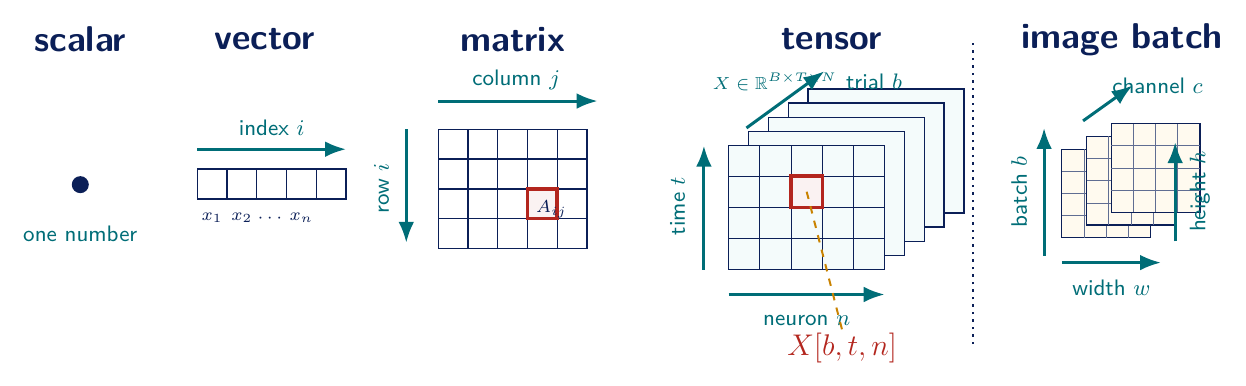
\includegraphics[width=0.96\linewidth]{imagegen-figures/ch07-tensor-shapes-axes.png}
\caption{Tensor notation extends scalar, vector, and matrix indexing to multi-axis arrays. The highlighted neural-recording entry \(X_{b,t,n}\) is specified by one index per axis: trial or batch \(b\), time \(t\), and neuron \(n\). In a deep learning image batch, the axes may be batch, height, width, and channel. The mathematical habit is to attach meaning to each axis before manipulating the array.}
\label{fig:ch07-tensor-shapes-axes}
\end{figure}

\paragraph{Formal setup.}
An order-\(d\) array over the real numbers has a shape
\[
I_1\times I_2\times\cdots\times I_d
\]
and is written
\[
A\in\mathbb{R}^{I_1\times I_2\times\cdots\times I_d}.
\]
Its entries are
\[
A_{i_1,i_2,\ldots,i_d},
\qquad
1\leq i_\ell\leq I_\ell\quad\text{for }\ell=1,\ldots,d.
\]
The number \(d\) is the order or number of axes. Be careful with the word ``rank'': in numerical computing people sometimes say ``rank'' to mean number of axes, while in linear algebra matrix rank means dimension of a column space. This chapter uses \emph{order} for the number of axes.

The \emph{mode} of a tensor is one of its axes. A mode-\(\ell\) fiber is obtained by fixing every index except \(i_\ell\). For example, if
\[
X\in\mathbb{R}^{B\times T\times N},
\]
with batch or trial index \(b\), time index \(t\), and neuron index \(n\), then \(X_{b,t,:}\in\mathbb{R}^N\) is the neural population vector at one trial and time.

The central equation of this section is simply the typed indexing rule:
\[
X\in\mathbb{R}^{B\times T\times N}
\quad\Longrightarrow\quad
X_{b,t,n}\in\mathbb{R}
\quad
(1\leq b\leq B,\ 1\leq t\leq T,\ 1\leq n\leq N).
\]
Every later tensor operation will be checked against this rule.

\paragraph{Core intuition.}
Figure~\ref{fig:ch07-tensor-shapes-axes} shows why tensors are not merely bigger matrices. A matrix has row and column axes. A three-way tensor has three independent directions of movement through the data. If the axes are trial \(b\), time \(t\), and neuron \(n\), then moving along the time axis asks how one trial evolves, moving along the neuron axis asks for a population pattern at one time, and moving along the trial axis asks how repeated measurements vary.

It is tempting to flatten every tensor into one long vector. Sometimes that is useful, especially because any finite array can be reshaped into a vector. But flattening discards visible axis structure. A \(20\times 100\times 50\) neural tensor has \(100{,}000\) numbers, just like a vector in \(\mathbb{R}^{100000}\). The tensor view remembers that those numbers came from 20 trials, 100 time bins, and 50 neurons. That memory determines which averages, filters, decoders, and plots are meaningful.

Common beginner misconceptions are shape misconceptions. First, the number of entries is not the same as the shape. Arrays of shape \((2,12)\), \((3,8)\), and \((2,3,4)\) all have 24 entries, but they support different axis-wise interpretations. Second, an axis is not always a spatial direction. Batch, time, neuron, token, frequency, and channel axes are all common. Third, reshaping is not automatically harmless. It is harmless only when the new shape preserves the intended correspondence between entries.

This section extends Chapter 4's matrix shape discipline. It prepares tensor contractions, deep learning layers, automatic differentiation, convolution, and population data analysis.

\paragraph{Main theorem: finite tensors can be vectorized, but shape carries extra structure.}
Every tensor
\[
A\in\mathbb{R}^{I_1\times\cdots\times I_d}
\]
can be placed in one-to-one correspondence with a vector in
\[
\mathbb{R}^{I_1I_2\cdots I_d}.
\]
However, that vectorization does not preserve axis meaning unless a specific indexing convention is recorded.

\emph{Proof sketch.} A tensor entry is identified by a multi-index
\[
(i_1,\ldots,i_d),
\qquad 1\leq i_\ell\leq I_\ell.
\]
There are \(I_1I_2\cdots I_d\) legal multi-indices. Choose a lexicographic ordering, for example with the last index changing fastest, and map
\[
(i_1,\ldots,i_d)
\quad\mapsto\quad
r
=1+\sum_{\ell=1}^d (i_\ell-1)\prod_{q=\ell+1}^d I_q.
\]
This assigns a unique vector coordinate \(r\) to every tensor entry. The inverse mapping recovers the multi-index by repeated division with remainders. Thus the entries can be vectorized without loss of numerical information.

The warning is conceptual rather than algebraic. The vector coordinate \(r\) does not say which original axis was trial, time, neuron, row, column, token, or channel. Tensor notation keeps those roles visible.

\paragraph{Worked examples.}
\emph{Small numerical example.} Let \(X\in\mathbb{R}^{2\times 3\times 2}\) have axes trial, time, and neuron. One legal entry is \(X_{2,1,2}\). The expression \(X_{3,1,2}\) is illegal because the first axis has length 2. The slice \(X_{2,1,:}\in\mathbb{R}^2\) is the two-neuron response vector on trial 2 at time 1, while \(X_{:,1,2}\in\mathbb{R}^2\) is the response of neuron 2 at time 1 across both trials.

\emph{ML/neuroscience example.} A minibatch of color images may be stored as
\[
X\in\mathbb{R}^{B\times H\times W\times C},
\]
where \(B\) is batch size, \(H\) is height, \(W\) is width, and \(C=3\) is color channel. A neural population data set may be stored as
\[
R\in\mathbb{R}^{B\times T\times N},
\]
where \(B\) is trial, \(T\) is time, and \(N\) is neuron. In both cases, the first axis indexes independent examples, but the remaining axes mean different things. A convolution over \(H,W\) is not the same operation as a temporal filter over \(T\), even if the arrays have the same number of entries.

\paragraph{ML/DL/neuroscience connections.}
In deep learning, the tensor is the basic runtime object. A linear layer often maps an activation tensor from shape \(B\times d_{\mathrm{in}}\) to \(B\times d_{\mathrm{out}}\). A convolutional layer maps \(B\times H\times W\times C_{\mathrm{in}}\) to \(B\times H'\times W'\times C_{\mathrm{out}}\). A transformer attention block maps a tensor with batch, token, and feature axes into another tensor with the same token structure but mixed information.

In neuroscience, tensors make population recordings explicit. A tensor \(R_{b,t,n}\) stores trial-by-time-by-neuron activity. Averaging over \(b\) estimates a trial-average response. Multiplying over the neuron axis by decoder weights forms a low-dimensional latent signal. Filtering over \(t\) extracts temporal structure. These are different operations because the axes have different meanings.

\paragraph{Exercises.}
\begin{enumerate}[label=\textbf{7.1.\arabic*.}, leftmargin=*]
\item \textbf{Mechanical.} For \(X\in\mathbb{R}^{4\times 5\times 3}\), list the legal ranges of all three indices. State the shapes of \(X_{2,:,:}\), \(X_{:,4,:}\), and \(X_{2,4,:}\).
\item \textbf{Proof or derivation.} For \(A\in\mathbb{R}^{I\times J\times K}\), derive a vectorization index \(r\) when the \(k\)-index changes fastest, then the \(j\)-index, then the \(i\)-index.
\item \textbf{Numerical/computational.} A tensor \(R\) has shape trial \(\times\) time \(\times\) neuron \(=30\times 100\times 64\). How many scalar entries does it contain? What is the shape after averaging over trials?
\item \textbf{Interpretation.} Explain why flattening \(R\in\mathbb{R}^{30\times 100\times 64}\) into a vector is numerically possible but may hide the difference between temporal structure and population structure.
\item \textbf{Debug the misconception.} A student says, ``Two arrays with the same number of entries are the same kind of input to a model.'' Give a shape-based counterexample involving images or neural recordings.
\end{enumerate}

\subsection{7.2 Tensor operations}

\paragraph{Motivating question.}
Once an array has several axes, which operations combine axes, preserve axes, reorder axes, or sum axes away?

\paragraph{Beginner setup.}
Tensor operations are rules for manipulating multi-index objects while respecting their shapes. Some operations create new axes. Some transform one axis while leaving others alone. Some reorder axes. Some sum over a shared axis and remove it from the result.

The smallest familiar example is matrix multiplication. If
\[
A\in\mathbb{R}^{m\times k},
\qquad
B\in\mathbb{R}^{k\times n},
\]
then
\[
C=AB\in\mathbb{R}^{m\times n}
\]
has entries
\[
C_{ij}=\sum_{\ell=1}^k A_{i\ell}B_{\ell j}.
\]
The shared \(\ell\)-axis is summed over and disappears. The unshared \(i\)- and \(j\)-axes remain. That is a tensor contraction.

Tensor operations solve the problem of writing array computations without flattening everything into one vector. They let us say exactly which axis is being mixed, copied, broadcast, permuted, or summed.

What to keep in mind: every operation has a shape contract. Before computing values, identify the input axes, the summed axes, and the output axes.

\begin{figure}[htbp]
\centering
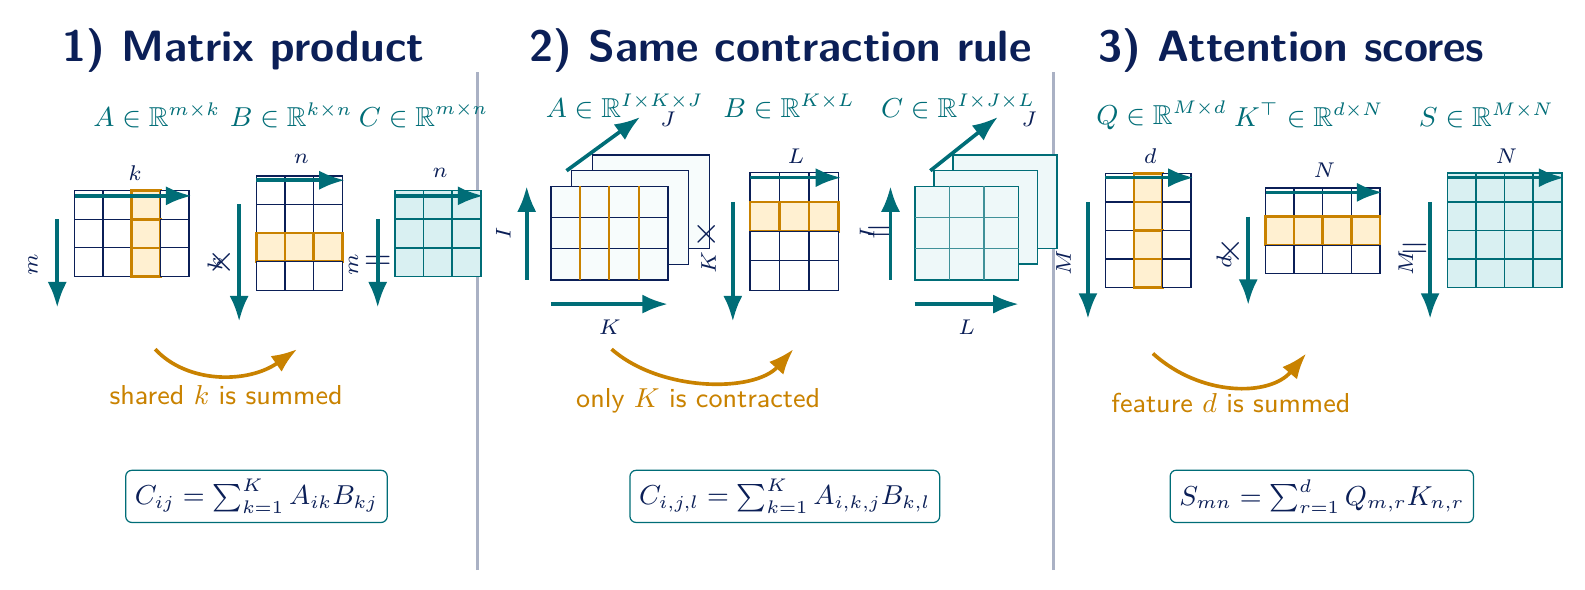
\includegraphics[width=0.98\linewidth]{imagegen-figures/ch07-contraction-einsum.png}
\caption{A contraction sums over a shared index and removes that index from the output. Matrix multiplication contracts over \(k\). The middle panel mirrors the formal higher-order example \(C_{i,j,l}=\sum_{k=1}^K A_{i,k,j}B_{k,l}\): only the \(K\)-axis is summed, while \(I,J,L\) remain. Attention scores \(S=QK^\top\) contract over the feature dimension \(d\), leaving query and key-token axes.}
\label{fig:ch07-contraction-einsum}
\end{figure}

\paragraph{Formal setup.}
Let
\[
A\in\mathbb{R}^{I_1\times\cdots\times I_p},
\qquad
B\in\mathbb{R}^{J_1\times\cdots\times J_q}.
\]
The \emph{outer product} creates a tensor with all axes from both inputs:
\[
(A\otimes B)_{i_1,\ldots,i_p,j_1,\ldots,j_q}
=A_{i_1,\ldots,i_p}B_{j_1,\ldots,j_q}.
\]
For vectors \(u\in\mathbb{R}^m\) and \(v\in\mathbb{R}^n\), this is the matrix
\[
(u\otimes v)_{ij}=u_i v_j.
\]

A \emph{contraction} multiplies entries and sums over one or more shared indices. For example, if
\[
A\in\mathbb{R}^{I\times K\times J},
\qquad
B\in\mathbb{R}^{K\times L},
\]
then contracting over \(k\) gives
\[
C_{i,j,l}
=\sum_{k=1}^{K}A_{i,k,j}B_{k,l},
\qquad
C\in\mathbb{R}^{I\times J\times L}.
\]
The contracted \(K\)-axis disappears; the uncontracted axes \(I,J,L\) remain.

A \emph{mode-\(r\) multiplication} applies a matrix to one axis of a tensor. If
\[
A\in\mathbb{R}^{I_1\times\cdots\times I_r\times\cdots\times I_d},
\qquad
M\in\mathbb{R}^{J\times I_r},
\]
then \(B=A\times_r M\) has shape
\[
I_1\times\cdots\times J\times\cdots\times I_d
\]
and entries
\[
B_{i_1,\ldots,j,\ldots,i_d}
=\sum_{i_r=1}^{I_r}
M_{j,i_r}A_{i_1,\ldots,i_r,\ldots,i_d}.
\]

Permutation reorders axes without changing entries, reshape changes the grouping of entries after choosing an ordering, and broadcasting copies a size-one axis across a larger compatible axis. The safest way to specify contractions is with explicit indices or with einsum notation, such as
\[
\texttt{ij,jk->ik}
\]
for matrix multiplication.

\paragraph{Core intuition.}
Figure~\ref{fig:ch07-contraction-einsum} gives the central visual rule. An index that appears in both inputs and is summed over is a consumed axis. An index that appears in the output is a surviving axis. Matrix multiplication is not a special trick; it is the simplest contraction most students already know.

Different operations answer different questions. The outer product asks for all pairwise combinations of two objects. A contraction asks for an alignment or weighted sum along a shared axis. Mode multiplication asks us to apply a matrix to every fiber along one axis. Transposition or permutation asks us to change axis order so that a later operation sees the intended dimensions. Broadcasting asks us to reuse values along an axis without explicitly storing copies.

Common misconceptions are again shape mistakes. First, reshaping is not the same as transposing: reshape changes how a linear list of entries is grouped, while transpose swaps axes. Second, broadcasting is not a mathematical sum; it silently repeats an array along a compatible axis. Third, a contraction requires matching dimensions on the summed index. If one object has a feature axis of length 64 and another has a feature axis of length 65, the contraction is not defined without another map.

This section extends matrix multiplication from Chapter 4. It prepares attention mechanisms, tensor decompositions, neural decoders, covariance summaries, and automatic differentiation systems that implement these operations at scale.

\paragraph{Main derivation: contraction as ``outer product plus summation''.}
Let \(A\in\mathbb{R}^{I\times K}\) and \(B\in\mathbb{R}^{K\times J}\). Their outer product has entries
\[
D_{i,k,k',j}=A_{i,k}B_{k',j}
\]
and shape \(I\times K\times K\times J\). Matrix multiplication keeps only matched pairs \(k=k'\) and sums over that shared index:
\[
C_{ij}
=\sum_{k=1}^K D_{i,k,k,j}
=\sum_{k=1}^K A_{i,k}B_{k,j}.
\]
This explains the mechanism. A contraction first pairs entries along compatible axes, then sums over the paired index. The output shape is obtained by deleting the summed index and retaining the free indices.

The same logic gives attention scores. If \(Q\in\mathbb{R}^{M\times d}\) contains query vectors and \(K\in\mathbb{R}^{N\times d}\) contains key vectors, then
\[
S=QK^\top\in\mathbb{R}^{M\times N},
\qquad
S_{mn}=\sum_{r=1}^d Q_{m,r}K_{n,r}.
\]
The feature index \(r\) is contracted, leaving query-token and key-token axes.

\paragraph{Worked examples.}
\emph{Small numerical example.} Let
\[
A=
\begin{bmatrix}
1&2\\
3&4
\end{bmatrix},
\qquad
B=
\begin{bmatrix}
5&6\\
7&8
\end{bmatrix}.
\]
Then
\[
C_{12}
=\sum_{k=1}^2 A_{1k}B_{k2}
=A_{11}B_{12}+A_{12}B_{22}
=1\cdot 6+2\cdot 8=22.
\]
The full product is
\[
AB=
\begin{bmatrix}
19&22\\
43&50
\end{bmatrix}.
\]
The index \(k\) was summed away; indices \(i,j\) survived.

\emph{ML/neuroscience example.} Let
\[
R\in\mathbb{R}^{B\times T\times N}
\]
store neural activity over trials, time, and neurons, and let \(w\in\mathbb{R}^N\) be decoder weights for one latent variable. The contraction
\[
z_{b,t}=\sum_{n=1}^N R_{b,t,n}w_n
\]
produces \(z\in\mathbb{R}^{B\times T}\). It keeps trial and time axes while summing over neurons. In einsum notation this is
\[
\texttt{btn,n->bt}.
\]
The mathematical operation is exactly a weighted population readout applied at every trial and time.

\paragraph{ML/DL/neuroscience connections.}
Many deep learning operations are contractions with carefully chosen axes. A fully connected layer applied to a batch is
\[
Y_{b,o}=\sum_i X_{b,i}W_{o,i}+b_o,
\]
which keeps the batch axis and contracts the input-feature axis. Attention scores contract query and key feature axes. A bilinear model contracts two feature vectors through a matrix:
\[
s=x^\top A y=\sum_{i,j}x_iA_{ij}y_j.
\]

In neuroscience, contractions turn large recordings into interpretable summaries. Contracting \(R_{b,t,n}\) with decoder weights over \(n\) gives a latent trajectory. Contracting over trials gives a mean time course. Contracting over time with a temporal basis function gives a response amplitude per trial and neuron. The index tells us what is being removed and what remains available for interpretation.

\paragraph{Exercises.}
\begin{enumerate}[label=\textbf{7.2.\arabic*.}, leftmargin=*]
\item \textbf{Mechanical.} For \(A\in\mathbb{R}^{3\times 4\times 5}\) and \(v\in\mathbb{R}^4\), define \(B_{i,k}=\sum_{j=1}^4 A_{i,j,k}v_j\). What is the shape of \(B\), and which axis was contracted?
\item \textbf{Proof or derivation.} Show that matrix multiplication \(C_{ij}=\sum_k A_{ik}B_{kj}\) is linear in \(A\) when \(B\) is fixed and linear in \(B\) when \(A\) is fixed.
\item \textbf{Numerical/computational.} Write einsum strings for these operations: matrix multiplication \(A_{ik}B_{kj}\), batch dot products \(X_{b,d}Y_{b,d}\to s_b\), and neural decoding \(R_{b,t,n}w_n\to z_{b,t}\).
\item \textbf{Interpretation.} In attention scores \(S_{mn}=\sum_r Q_{m,r}K_{n,r}\), what do the surviving indices \(m,n\) mean, and what information is removed by summing over \(r\)?
\item \textbf{Debug the misconception.} A student says, ``Broadcasting a vector over a batch is the same as taking an average over the batch.'' Explain the difference between copying along an axis and summing over an axis.
\end{enumerate}

\subsection{7.3 Matrix and tensor derivatives}

\paragraph{Motivating question.}
When a computation maps vectors, matrices, or tensors to other arrays, what shape should its derivative have?

\paragraph{Beginner setup.}
Derivatives measure local change. For scalar functions of one variable, the derivative is a number. For functions of many variables, the derivative must describe how every output changes when every input coordinate is perturbed. Shape-first matrix calculus is the habit of asking for the shape of the derivative before writing formulas.

The smallest multivariable example is a scalar loss
\[
L:\mathbb{R}^n\to\mathbb{R}.
\]
Its gradient \(\nabla_x L\in\mathbb{R}^n\) has the same shape as \(x\). The first-order change is
\[
dL=(\nabla_x L)^\top dx.
\]
If instead
\[
f:\mathbb{R}^n\to\mathbb{R}^m,
\]
then the derivative is the Jacobian
\[
J_f(x)\in\mathbb{R}^{m\times n},
\qquad
(J_f)_{ij}=\frac{\partial f_i}{\partial x_j},
\]
and the local change is
\[
df=J_f(x)\,dx.
\]

Matrix and tensor derivatives solve the problem that models have many parameters arranged in meaningful shapes. A weight matrix \(W\) should receive a gradient shaped like \(W\), not a mysterious vector whose coordinates have to be decoded later.

What to keep in mind: for a scalar loss, the gradient with respect to an array has the same shape as that array. For an array-valued function, the full derivative has output axes and input axes.

\begin{figure}[htbp]
\centering
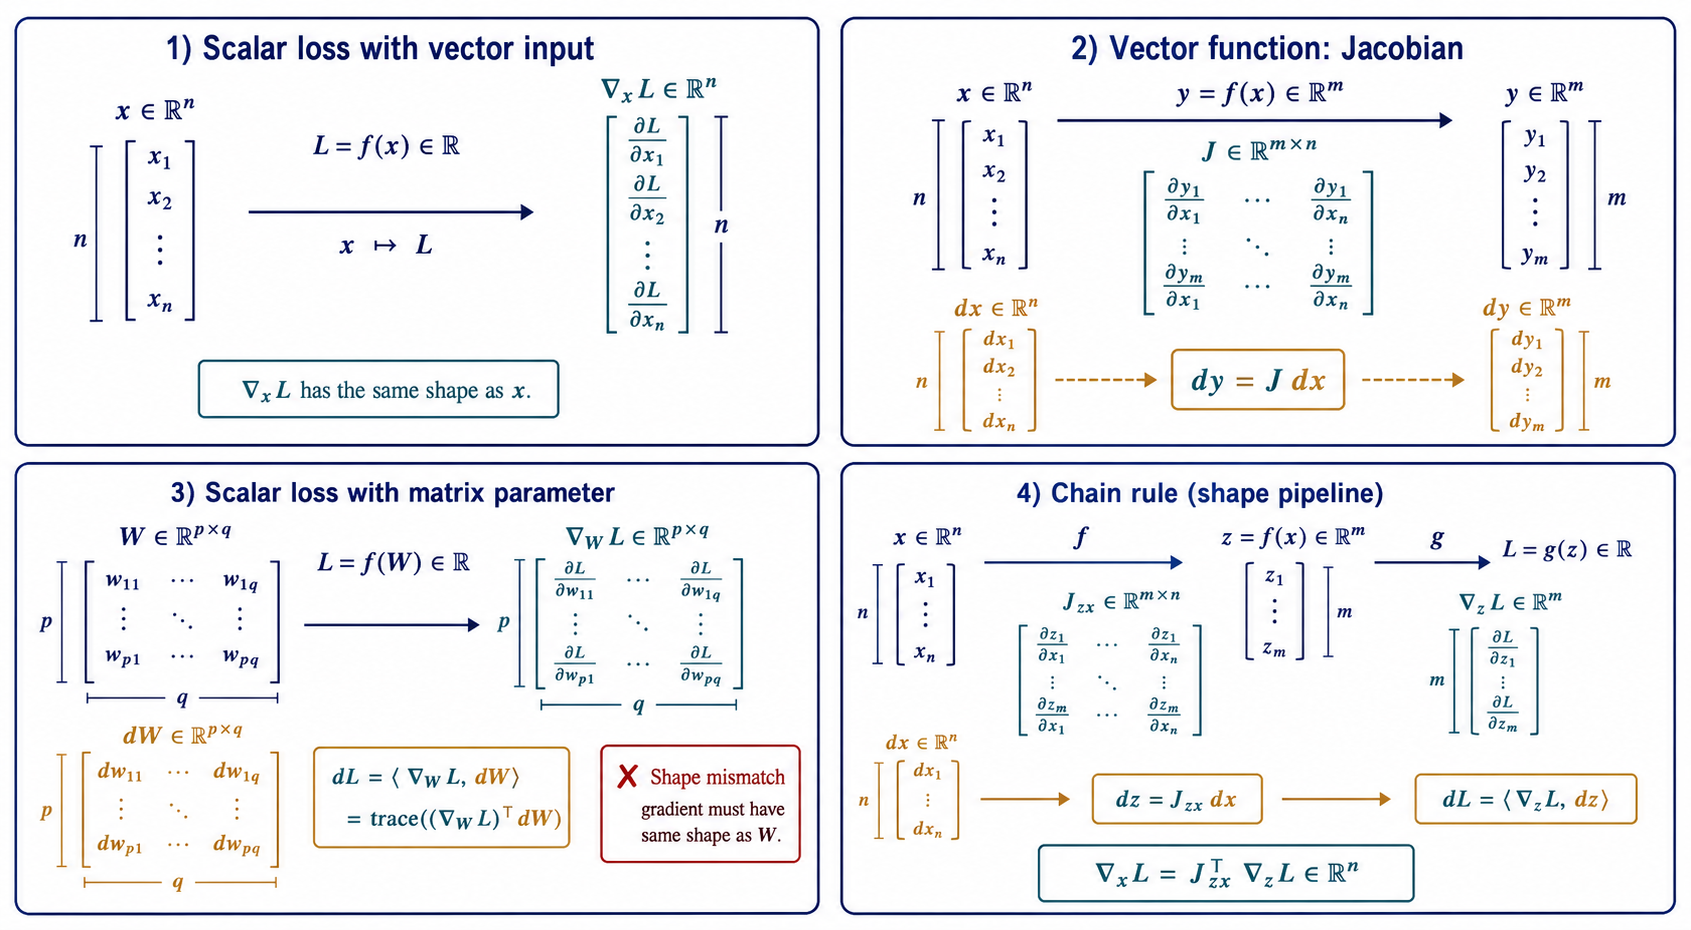
\includegraphics[width=0.98\linewidth]{imagegen-figures/ch07-shape-first-derivatives.png}
\caption{Shape-first derivatives keep domains and codomains visible. A scalar loss has a gradient with the same shape as its input. A vector-valued function has a Jacobian mapping input perturbations to output perturbations. A scalar loss with matrix parameter \(W\) has a matrix gradient paired with \(dW\) through the Frobenius inner product. Chain rules transpose Jacobians when moving gradients backward.}
\label{fig:ch07-shape-first-derivatives}
\end{figure}

\paragraph{Formal setup.}
We use numerator-layout Jacobians:
\[
f:\mathbb{R}^n\to\mathbb{R}^m,
\qquad
J_f(x)_{ij}=\frac{\partial f_i}{\partial x_j},
\qquad
df=J_f(x)\,dx.
\]
For a scalar loss \(L:\mathbb{R}^n\to\mathbb{R}\),
\[
dL=(\nabla_x L)^\top dx,
\qquad
\nabla_x L\in\mathbb{R}^n.
\]
For a scalar loss depending on a matrix
\[
L:\mathbb{R}^{p\times q}\to\mathbb{R},
\]
the gradient is defined by the Frobenius pairing
\[
dL=\langle \nabla_W L,dW\rangle_F
=\operatorname{tr}\big((\nabla_W L)^\top dW\big),
\qquad
\nabla_W L\in\mathbb{R}^{p\times q}.
\]
For a tensor parameter
\[
\Theta\in\mathbb{R}^{I_1\times\cdots\times I_d},
\]
the scalar-loss gradient \(\nabla_\Theta L\) has the same shape, with entries
\[
(\nabla_\Theta L)_{i_1,\ldots,i_d}
=\frac{\partial L}{\partial \Theta_{i_1,\ldots,i_d}}.
\]
For example, if
\[
L(\Theta)=\frac12
\sum_{b=1}^B\sum_{t=1}^T\sum_{n=1}^N
(\Theta_{b,t,n}-Y_{b,t,n})^2,
\qquad
\Theta,Y\in\mathbb{R}^{B\times T\times N},
\]
then each entry differentiates independently:
\[
(\nabla_\Theta L)_{b,t,n}=\Theta_{b,t,n}-Y_{b,t,n}.
\]
So \(\nabla_\Theta L=\Theta-Y\), with the same trial-by-time-by-neuron shape as \(\Theta\).

The Hessian of a scalar function \(L:\mathbb{R}^n\to\mathbb{R}\) is
\[
H_{ij}=\frac{\partial^2 L}{\partial x_i\partial x_j},
\qquad
H\in\mathbb{R}^{n\times n}.
\]
It is the Jacobian of the gradient and controls local curvature:
\[
d(\nabla_x L)=H\,dx.
\]
For least squares,
\[
L(x)=\frac12\|Ax-b\|^2,
\qquad
\nabla_x L=A^\top(Ax-b).
\]
Differentiating the gradient gives
\[
d(\nabla_x L)=A^\top A\,dx,
\]
so the Hessian is
\[
\nabla_x^2 L=A^\top A\in\mathbb{R}^{n\times n}.
\]

\paragraph{Core intuition.}
Figure~\ref{fig:ch07-shape-first-derivatives} shows the two roles derivatives play. Forward derivatives push perturbations forward: \(dx\mapsto dy\). Backward derivatives pull loss gradients backward: \(\nabla_y L\mapsto \nabla_x L\). Those two views are related by transposition.

Differentials are useful because they make shapes hard to fake. If \(y=Wx\) with \(W\in\mathbb{R}^{m\times n}\), then
\[
dy=dW\,x+W\,dx.
\]
The term \(dW\,x\) has shape \(m\), and \(W\,dx\) has shape \(m\). If a proposed formula produces a vector of shape \(n\) at this stage, it cannot be right.

Common misconceptions come from memorizing formulas without domains. First, the gradient of a scalar loss with respect to a matrix is a matrix, not a row vector unless one explicitly vectorizes. Second, the Jacobian of \(f:\mathbb{R}^n\to\mathbb{R}^m\) is \(m\times n\) under the convention used here, because it maps \(dx\in\mathbb{R}^n\) to \(df\in\mathbb{R}^m\). Third, \(A^\top A\) appears in least squares derivatives because the residual is first pushed forward by \(A\) and then pulled back by \(A^\top\).

This section formalizes the derivative habits that deep learning frameworks automate. Automatic differentiation does not remove the need for shape reasoning; it makes shape reasoning more important because the computation graph may contain many arrays.

\paragraph{Main derivation: gradients from differentials and the chain rule.}
Consider the least-squares loss
\[
L(x)=\frac12\|Ax-b\|^2,
\qquad
A\in\mathbb{R}^{m\times n},
\quad x\in\mathbb{R}^n,
\quad b\in\mathbb{R}^m.
\]
Let
\[
r=Ax-b\in\mathbb{R}^m.
\]
Then
\[
L=\frac12 r^\top r.
\]
Differentiate in steps. The residual change is
\[
dr=A\,dx.
\]
The loss change is
\[
dL=r^\top dr.
\]
Substitute \(dr=A\,dx\):
\[
dL=r^\top A\,dx.
\]
Move parentheses so the coefficient of \(dx\) is visible:
\[
dL=(A^\top r)^\top dx.
\]
By the definition \(dL=(\nabla_x L)^\top dx\), we get
\[
\nabla_x L=A^\top(Ax-b).
\]
The shape is correct: \(A^\top\in\mathbb{R}^{n\times m}\) pulls the residual \(r\in\mathbb{R}^m\) back to \(\mathbb{R}^n\).
Differentiating once more,
\[
d(\nabla_x L)=A^\top A\,dx,
\]
so the Hessian is
\[
\nabla_x^2L=A^\top A.
\]
This matrix has shape \(n\times n\), matching a linear map from an input perturbation \(dx\in\mathbb{R}^n\) to a gradient perturbation.

For a linear layer with one example,
\[
y=Wx+b,
\qquad
W\in\mathbb{R}^{m\times n},
\quad x\in\mathbb{R}^n,
\quad y\in\mathbb{R}^m,
\]
let \(g=\nabla_y L\in\mathbb{R}^m\). Since
\[
dy=dW\,x+W\,dx+db,
\]
the loss differential is
\[
dL=g^\top dy
=g^\top dW\,x+g^\top W\,dx+g^\top db.
\]
The \(W\)-term is a scalar, so we may write it as a trace and rotate the factors cyclically:
\[
g^\top dW\,x
=\operatorname{tr}(g^\top dW\,x)
=\operatorname{tr}(xg^\top dW)
=\operatorname{tr}\big((gx^\top)^\top dW\big)
=\langle gx^\top,dW\rangle_F.
\]
This last line matches the defining form
\[
dL=\langle \nabla_W L,dW\rangle_F+\cdots.
\]
The three gradients are therefore
\[
\nabla_x L=W^\top g,
\qquad
\nabla_b L=g,
\qquad
\nabla_W L=gx^\top.
\]
The matrix gradient \(gx^\top\) has shape \(m\times n\), the same as \(W\).

The vector chain rule follows the same mechanism. If \(z=f(x)\in\mathbb{R}^m\) and \(L=g(z)\in\mathbb{R}\), then
\[
dz=J_f(x)\,dx,
\qquad
dL=(\nabla_z L)^\top dz.
\]
Substitute:
\[
dL=(\nabla_z L)^\top J_f(x)\,dx
=\big(J_f(x)^\top\nabla_z L\big)^\top dx.
\]
Thus
\[
\nabla_x L=J_f(x)^\top\nabla_z L.
\]
This is the local algebra behind backpropagation.

\paragraph{Worked examples.}
\emph{Small numerical example.} Let
\[
A=
\begin{bmatrix}
1&2\\
0&1\\
3&0
\end{bmatrix},
\qquad
x=
\begin{bmatrix}
1\\
-1
\end{bmatrix},
\qquad
b=
\begin{bmatrix}
0\\
1\\
2
\end{bmatrix}.
\]
Then
\[
Ax=
\begin{bmatrix}
-1\\
-1\\
3
\end{bmatrix},
\qquad
r=Ax-b=
\begin{bmatrix}
-1\\
-2\\
1
\end{bmatrix}.
\]
The gradient is
\[
\nabla_x L=A^\top r
=
\begin{bmatrix}
1&0&3\\
2&1&0
\end{bmatrix}
\begin{bmatrix}
-1\\
-2\\
1
\end{bmatrix}
=
\begin{bmatrix}
2\\
-4
\end{bmatrix}.
\]
It has the same shape as \(x\).

\emph{Tensor-gradient example.} Let \(\Theta,Y\in\mathbb{R}^{2\times 3\times 2}\) and
\[
L(\Theta)=\frac12\sum_{b,t,n}(\Theta_{b,t,n}-Y_{b,t,n})^2.
\]
The differential is
\[
dL=\sum_{b,t,n}(\Theta_{b,t,n}-Y_{b,t,n})\,d\Theta_{b,t,n}.
\]
Comparing with the tensor Frobenius pairing gives
\[
\nabla_\Theta L=\Theta-Y.
\]
Every gradient entry keeps the same trial, time, and neuron address as the parameter entry it differentiates.

\emph{ML/neuroscience example.} In a neural decoder, let \(x\in\mathbb{R}^N\) be one population response vector and \(W\in\mathbb{R}^{K\times N}\) map neural activity to \(K\) behavior scores. If the upstream gradient from the loss is \(g\in\mathbb{R}^K\), then
\[
\nabla_W L=gx^\top.
\]
Each weight update is an outer product between output error and input activity. This is one reason outer-product learning rules appear so often in both artificial networks and simplified models of synaptic plasticity.

\paragraph{ML/DL/neuroscience connections.}
Backpropagation is repeated application of the chain rule
\[
\nabla_x L=J^\top\nabla_y L.
\]
The Jacobian may be too large to form explicitly, but its action and transpose action are computed by automatic differentiation. A convolutional layer, attention layer, normalization layer, or recurrent update all has a local derivative that pushes perturbations forward and pulls gradients backward.

In neuroscience models, matrix and tensor derivatives appear when fitting encoding models, dynamical systems, GLMs, and latent-variable models. A loss over spike counts may depend on filters, coupling weights, and latent trajectories. The gradient with respect to each object must have that object's shape, because each entry represents a particular neuron, lag, feature, or time point.

\paragraph{Exercises.}
\begin{enumerate}[label=\textbf{7.3.\arabic*.}, leftmargin=*]
\item \textbf{Mechanical.} Let \(f:\mathbb{R}^3\to\mathbb{R}^2\). Under the Jacobian convention in this chapter, what is the shape of \(J_f\)? If \(dx\in\mathbb{R}^3\), what is the shape of \(df=J_fdx\)?
\item \textbf{Proof or derivation.} Derive \(\nabla_x \frac12\|Ax-b\|^2=A^\top(Ax-b)\) and \(\nabla_x^2\frac12\|Ax-b\|^2=A^\top A\) using differentials, stating the shape of every object.
\item \textbf{Numerical/computational.} For \(y=Wx+b\), with \(W\in\mathbb{R}^{4\times 3}\), \(x\in\mathbb{R}^3\), and upstream gradient \(g=\nabla_y L\in\mathbb{R}^4\), give the shapes of \(\nabla_W L\), \(\nabla_x L\), and \(\nabla_b L\). Then for \(\Theta,Y\in\mathbb{R}^{5\times 10\times 3}\) and \(L(\Theta)=\frac12\|\Theta-Y\|_F^2\), give the shape and entry formula for \(\nabla_\Theta L\). Write pseudocode for both computations.
\item \textbf{Interpretation.} In the formula \(\nabla_W L=gx^\top\), what do the row index and column index of the gradient correspond to in a linear neural decoder?
\item \textbf{Debug the misconception.} A student says, ``The derivative of a scalar loss is always just one number.'' Explain why that is true only for a scalar input variable, and give the gradient shape for \(L(W)\) with \(W\in\mathbb{R}^{p\times q}\).
\end{enumerate}

\subsection{7.4 Convolution as linear algebra}

\paragraph{Motivating question.}
How can a sliding filter be understood as a linear map with special sparse structure?

\paragraph{Beginner setup.}
Convolution combines a signal with a small kernel by sliding the kernel across locations and taking local weighted sums. In signal processing, convolution often includes a reversal of the kernel. In many deep learning libraries, the operation called convolution is technically cross-correlation because the kernel is not reversed. The distinction matters for exact formulas, but both are linear maps with the same shape discipline. We will use the convention
\[
y_t=\sum_{r=-R}^{R}h_r x_{t-r},
\]
with zero padding when an index \(t-r\) lies outside the signal.

The smallest useful example has a one-dimensional signal
\[
x=(x_1,x_2,x_3,x_4)
\]
and a three-tap kernel
\[
h=(-1,0,1),
\]
with entries \(h_{-1}=-1\), \(h_0=0\), and \(h_1=1\). Each output entry uses only nearby input entries. The kernel is reused at every location.

Convolution solves the problem of local pattern detection with shared weights. A small filter can detect the same feature at many locations without learning separate weights for every location. This is why convolution appears in image processing, CNNs, temporal filtering, and neural signal analysis.

What to keep in mind: convolution is linear in the input when the kernel is fixed. It is also linear in the kernel when the input is fixed. Its special power comes from sparsity, weight sharing, and translation equivariance, not from being nonlinear.

\begin{figure}[htbp]
\centering
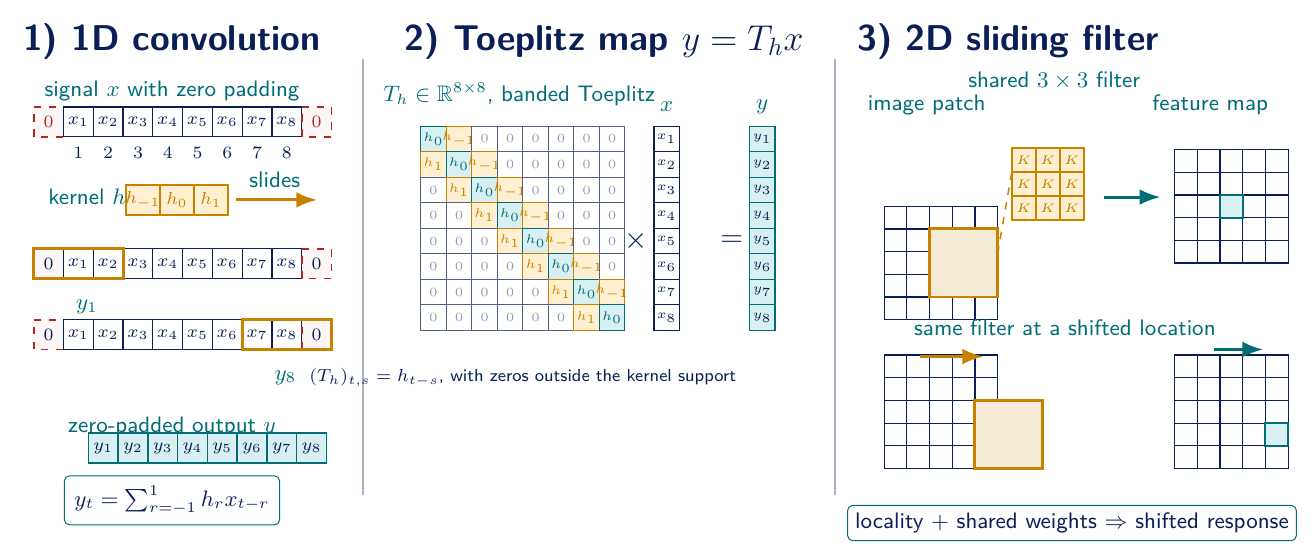
\includegraphics[width=0.98\linewidth]{imagegen-figures/ch07-convolution-toeplitz.png}
\caption{A convolution is a structured sparse linear map. In the one-dimensional \(N=8\) zero-padded schematic, the input \(x_1,\ldots,x_8\) produces eight outputs \(y_1,\ldots,y_8\). The same operation can be written as \(y=T_hx\), where \(T_h\in\mathbb{R}^{8\times 8}\) is a Toeplitz matrix whose diagonals contain shared kernel weights. In two dimensions, the same filter moves across an image to produce a feature map; shifting the input pattern shifts the output response.}
\label{fig:ch07-convolution-toeplitz}
\end{figure}

\paragraph{Formal setup.}
Let \(x\in\mathbb{R}^N\) be a one-dimensional signal and let \(h\in\mathbb{R}^{2R+1}\) be a kernel indexed by \(r=-R,\ldots,R\). With zero padding, define
\[
y_t=\sum_{r=-R}^{R}h_r x_{t-r},
\qquad t=1,\ldots,N,
\]
where \(x_s=0\) if \(s\notin\{1,\ldots,N\}\). This defines a linear map
\[
T_h:\mathbb{R}^N\to\mathbb{R}^N,
\qquad
y=T_hx.
\]
The matrix \(T_h\) is Toeplitz: entries are constant along diagonals. Specifically,
\[
(T_h)_{t,s}=h_{t-s}
\]
when \(t-s\in\{-R,\ldots,R\}\), and zero otherwise. The nonzero pattern is banded because each output depends only on nearby inputs.

Stride keeps every \(s\)th output location instead of every location. Padding controls how boundary indices outside the original signal are treated. In two dimensions, for an image \(X\in\mathbb{R}^{H\times W}\) and kernel \(K\in\mathbb{R}^{(2R+1)\times(2S+1)}\),
\[
Y_{p,q}=\sum_{r=-R}^{R}\sum_{s=-S}^{S}K_{r,s}X_{p-r,q-s}.
\]
With channels, a convolutional layer also sums over input channels and produces output channels:
\[
Y_{b,p,q,o}
=\sum_{r,s,i}K_{r,s,i,o}X_{b,p-r,q-s,i},
\]
where \(b\) indexes batch, \(p,q\) index spatial position, \(i\) indexes input channel, and \(o\) indexes output channel.

\paragraph{Core intuition.}
Figure~\ref{fig:ch07-convolution-toeplitz} shows two equivalent views. The sliding-kernel view is local and visual: the same weights move across the signal. The matrix view is algebraic: the operation is multiplication by a sparse matrix with repeated diagonal entries. The repeated entries are weight sharing. The zeros are locality.

Translation equivariance means that shifting the input shifts the output in the same way, away from boundaries. If a vertical edge appears on the left side of an image, a filter can respond there. If the same edge appears on the right side, the same filter responds on the right side. The operation does not need new weights for the new location.

Common misconceptions are common because convolution is introduced in many contexts. First, convolution is not automatically nonlinear. A CNN becomes nonlinear because convolution is followed by nonlinearities such as ReLU. Second, a convolutional layer is not just a matrix with fewer parameters; it is a matrix whose entries are tied together according to a spatial or temporal pattern. Third, padding is not mathematically invisible. Boundary behavior changes the linear map.

This section connects tensor operations to later function-space and deep learning chapters. In Chapter 12, convolution becomes an operator on functions and relates to Fourier transforms. In deep learning, convolution becomes a learnable tensor contraction with shared local weights.

\paragraph{Main theorem: fixed-kernel convolution is linear and translation equivariant.}
For a fixed kernel \(h\), the map \(T_h:x\mapsto h*x\) defined by
\[
(T_hx)_t=\sum_r h_r x_{t-r}
\]
is linear. On an infinite or periodic signal domain, it is translation equivariant: if \(S_a\) shifts a signal by \(a\), then
\[
T_h(S_a x)=S_a(T_hx).
\]

\emph{Proof sketch.} Linearity follows from distributing the sum. For signals \(x,z\) and scalars \(\alpha,\beta\),
\[
T_h(\alpha x+\beta z)_t
=\sum_r h_r(\alpha x_{t-r}+\beta z_{t-r})
=\alpha\sum_r h_rx_{t-r}+\beta\sum_r h_rz_{t-r}.
\]
Thus
\[
T_h(\alpha x+\beta z)=\alpha T_hx+\beta T_hz.
\]

For equivariance, define \((S_a x)_t=x_{t-a}\). Then
\[
(T_h(S_a x))_t
=\sum_r h_r(S_a x)_{t-r}
=\sum_r h_rx_{t-r-a}.
\]
On the other hand,
\[
(S_a(T_hx))_t
=(T_hx)_{t-a}
=\sum_r h_rx_{t-a-r}.
\]
The expressions are the same. Boundaries can break exact equivariance, which is why padding conventions matter.

\paragraph{Worked examples.}
\emph{Small numerical example.} Let \(x=(1,2,0,1)\) and \(h_{-1}=-1\), \(h_0=0\), \(h_1=1\), with zero padding. Then
\[
y_t=-x_{t+1}+x_{t-1}.
\]
The outputs are
\[
y_1=-x_2+x_0=-2+0=-2,
\]
\[
y_2=-x_3+x_1=0+1=1,
\]
\[
y_3=-x_4+x_2=-1+2=1,
\]
\[
y_4=-x_5+x_3=0+0=0.
\]
Thus \(y=(-2,1,1,0)\). The equivalent matrix is
\[
T_h=
\begin{bmatrix}
0&-1&0&0\\
1&0&-1&0\\
0&1&0&-1\\
0&0&1&0
\end{bmatrix},
\qquad
y=T_hx.
\]

\emph{ML/neuroscience example.} In a CNN, a \(3\times 3\) edge detector is applied at every image location. The image tensor supplies local patches, the kernel tensor supplies shared weights, and the output feature map stores local weighted sums. In neural data analysis, a temporal filter can be convolved with a spike train or local field potential to detect bursts, oscillations, or event-locked responses. In both cases, the operation is a structured linear map before any nonlinearity is applied.

\paragraph{ML/DL/neuroscience connections.}
A convolutional layer maps an input activation tensor to an output activation tensor by a local tensor contraction. The kernel entries are learned parameters. The local patch entries are data. The sum over offsets and input channels produces one output channel at one location. Weight sharing means the same kernel tensor is reused across spatial or temporal positions.

In neuroscience, receptive-field models are often convolutional in time or space. A linear-nonlinear model may first compute
\[
u_t=\sum_r h_r s_{t-r}
\]
from a stimulus \(s\), then pass \(u_t\) through a nonlinearity to predict firing rate. The kernel \(h\) is a temporal receptive field. The convolution is the linear filtering stage; the nonlinearity models the spike-rate transformation.

\paragraph{Exercises.}
\begin{enumerate}[label=\textbf{7.4.\arabic*.}, leftmargin=*]
\item \textbf{Mechanical.} For \(x=(2,1,3)\) and \(h_{-1}=1\), \(h_0=2\), \(h_1=0\), compute \(y_t=\sum_{r=-1}^1 h_rx_{t-r}\) with zero padding.
\item \textbf{Proof or derivation.} Write the Toeplitz matrix \(T_h\) for a length-5 signal and kernel \(h_{-1},h_0,h_1\) with zero padding. Explain why \(T_hx\) equals convolution.
\item \textbf{Numerical/computational.} Give pseudocode for a one-dimensional convolution with stride 2 and zero padding. State the output length for input length \(N=8\), kernel width 3, padding 1, and stride 2.
\item \textbf{Interpretation.} In a CNN, what do locality and weight sharing mean in the equivalent matrix representation?
\item \textbf{Debug the misconception.} A student says, ``Convolutional layers are nonlinear because CNNs are nonlinear.'' Separate the fixed-kernel convolution operation from the nonlinear activation that may follow it.
\end{enumerate}

The durable lesson of this chapter is shape discipline. Tensors keep axis structure visible. Contractions tell us exactly which axes are summed away. Matrix calculus makes derivative shapes explicit. Convolution shows that many familiar neural-network operations are ordinary linear maps with special structure.

Later chapters will reuse these ideas constantly. Multivariable calculus and optimization rely on Jacobians, gradients, and Hessians. Automatic differentiation is an organized chain rule over tensor programs. Deep networks are compositions of tensor contractions, nonlinearities, and structured linear maps. Neural population analysis treats recordings as trial-by-time-by-neuron arrays and uses contractions, filters, and low-dimensional projections to extract scientific structure.

\clearpage
